\section{Validation and best practices}
\label{sec:validation}
\subsection{Finding a balance between precision and recall}
\label{sec:balance}

In the previous sections, we have learned how to fit different models:
Na\"ive Bayes, logistic regressions, support vector machines, and
random forests.  We have also had a first look at confusion matrices,
precision, and recall.

But how do we find the best model? ``Best'', here, should be read as
``best for our purposes'' -- some models may be bad, and some may be
good, but which one is really the best may depend on what matters most
for us: Do we care more about precision or about recall? Are all
classes equally important to us?  And of course, other factors, such
as explainability or computational costs may factor into our decision.
 
But in any event, we need to decide which metrics to focus on.  We can
then either manually inspect them and look, for instance, which model
has the highest \emph{accuracy}, or the best balance of precision and recall,
or a recall higher than some threshold you are willing to accept.

If we build a classifier to distinguish spam messages from legitimate
messages, we could ask the following questions:
\begin{description}
\item[Precision] Which percentage of what our classifier predicts to be
  spam really is spam?
\item[Recall]{What percentage of all spam messages has our classifier
  found?}
\item[Accuracy]{In which percentage of all cases was our classifier
  right?}
\end{description}

We furthermore have:
\begin{description}
\item[F1-score]{The harmonic mean of precision and recall: $F_1 = 2
  \cdot \frac{precison \cdot recall}{precison + recall}$}
\item[AUC]{The AUC (Area under Curve) is the area under the curve that
  one gets when plotting the True Positive Rate (TPR) against the
  False Positive Rate (FPR) at various threshold settings. A perfect
  model will receive a value of 1.0, while random guessing between two
  equally probable classes will result in a value of 0.5}
\item[Micro- and macroaverage]{Especially when we have more than two
  classes, we can calculate the average of measures such as precision,
  recall, or f1-score. We can do so based on the separately calculated
  measures (macro), or based on the underlying values (TP, FP, etc.)
  (micro), which has different implications in the interpretation --
  especially if the classes have very different sizes.}
\end{description}


So, which one to choose?  If we really do not want to be annoyed by
any spam in our inbox, we need a high recall (we want to find all spam
messages). If, instead, we want to be sure that we do not
accidentally throw away legitimate messages, we need a high
precision (we want to be sure that all spam really is spam).

Maybe you say: well, I want both!  You could look at the accuracy, a
very straightforward to interpret measure. However, if you get many
more legitimate messages than spam (or the other way round), this
measure can be misleading: after all, even if your classifier finds
almost none of the spam messages (it has a recall close to zero), you
still get a very high accuracy, simply because there are so many
legitimate messages. In other words, the accuracy is not a good measure when working with highly unbalanced classes.
Often, it is therefore a better idea to look at the harmonic mean of
precision and recall, the F1-score, if you want to find a model that
gives you a good compromise between precision and recall.


In fact, we can even fine-tune our models in such a way that they are
geared towards either a better precision or a better recall.
As an example, let us take a logistic regression model. It predicts a
class label (such as ``spam'' versus ``legitimate''), but it can also
return the assigned probabilities. For a specific message, we can thus
say that we estimate its probability of being spam as, say, .65.
Unless we specify otherwise, everything above .5 will then be judged
to be spam, everything below as legitimate. But we could specify a
different cutoff point: we could, for instance, decide to classify
only everything above .7 as spam. This would give us a more
conservative spam filter, with probably a higher precision at the
expense of a lower recall.

\begin{figure} 
\centering
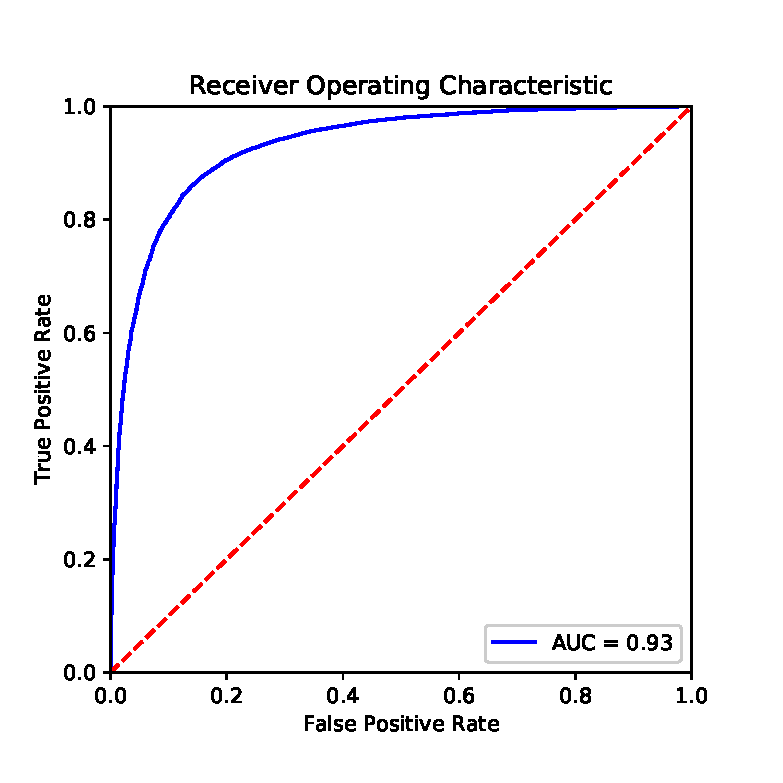
\includegraphics[width=0.4\linewidth]{figures/ch09_roccurve}
\caption{A (pretty good) ROC curve.}
\label{fig:roccurve}
\end{figure}

We can visualize this with a so-called ROC (reveicer operator
chraracteristic), a plot in which (Figure~\ref{fig:roccurve}) we plot
true positives against false positives at different thresholds.  A
good model extends until close to the upper left corner, and hence has
a large area under the curve (AUC).  If we choose a threshold at the
left end of the curve, we get few false positives (good!), but also
few true positives (bad!), if we go too far to the right, we get
the other extreme. So, how can we find the best spot?

\refex{cutoffpoint} provides two approaches. One approach is to print a table with three columns: the false
positive rate, the true positive rate, and the threshold value. You
then decide which FPR-TPR combination is most appealing to you, and
use the corresponding threshold value. Having calculated the TPR and FPR anyway, we can
also additionally plot them as ROC curve (\refex{roccurve}), which may help
us interpreting the table.
The second approach (also knwon as Yoden's J) is to find the threshold
value with the maximum distance between TPR and FPR, and use that one.

\pyrex[input=py, output=py,caption={Choosing a differnet cutoff point for predictions with logistic regression. In this case, we make a tradeoff and maximize the difference between false positive rate and true positive rate to improve the precision for the the second categegory by .12 at the expense of reducing the precision for the first category by .8.}]{chapter09/cutoffpoint}


\pyrex[input=py, output=py,format=png,caption={The ROC curve of a (not very impressive) classifier and its area under the curve (AUC)}]{chapter09/roccurve}



\subsection{Train, validate, test}
\label{sec:train}

By now, we have established which measures we can use to decide which
model to use. For all of them, we have assumed that we split our
labeled dataset into two: a training dataset and a test dataset. The
logic behind it was simple: If we would calculate precision and recall
on the training data itself, our assessment would be too optimistic --
after all, our models have been trained on exactly these data, so
predicting the label isn't too hard. Assessing the models on a different
dataset, the test dataset, instead, gives us an assessment of how
precision and recall look like if haven't seen the labels earlier --
which is exactly what we want to know.

Unfortunately, if we calculate precision and recall (or any other
metric) for multiple models on the same test dataset, and use these
results to determine which metric to use, we can run into a problem:
We may avoid overfitting of our model on the training data, we may now
overfit it on the test data! After all, we could tweak our models as
long until they fit our test data perfectly, even if this makes the
predictions for other cases worse.

One way to avoid this is to split the original data into three
datasets instead of two: a training dataset, a validation dataset, and
a test dataset.  We train multiple model configurations on the
training dataset and calculate the metrics of interest for all of them
on the validation dataset.  Once we have decided on a final model, we
calculate its performance (once) on the test dataset, to get an
unbiased estimate of its performance.



\subsection{Cross-validation and grid search}
\label{sec:crossvalidation}
In an ideal world, we would have a huge labelled dataset and do not
need to worry about the decreasing size of our training dataset as we
set aside our validation and test datasets.

Unfortunately, our labelled datasets in the real world have a limited
size, and setting aside too many cases can be problematic. Especially
if you are already on a tight budget, setting aside not only a test
dataset, but also a validation dataset of meaningful size may lead to
critically small training datasets. While we have addressed the
problem of overfitting, this could lead to underfitting: We may have
removed the only examples of some specific feature combination, for
instance.

A common approach to address this issue is $k$-fold
cross-validation. To do so, we split our data into $k$ partitions,
so-called folds. We then estimate our model $k$ times, and each time
leave \emph{one} of the folds aside for validation. Hence, every fold
is exactly one time the validation dataset, and exactly $k-1$ times
part of the training data. We then simply average the results of our
$k$ values for the evaluation metric we are interested in.

If our classifier generalizes well, we would expect that our metric of
interest (e.g., the accuracy, or the f1-score, \ldots) is very similar
in all folds. ~\refex{crossval} performs a cross-validation based on
the logistic regression classifier we build above. We see that the
standard deviation is really low, indicating that there are almost no
changes between the runs, which is great.

Running the same cross-validation on our random forest, instead, would
produce not only worse (lower) means, but also worse (higher) standard
deviations, even though also here, there are no dramatic changes
between the runs.

\pyrex[input=both, output=both,caption=Crossvalidation]{chapter09/crossval}

Very often, cross-validation is used when we want to compare many
different model specifications, for example to find optimal
hyperparameters.
Hyperparameters are parameters of the model that are not estimated
from the data. These depend on the model, but could for example be the
estimation method to use, the number of times a bootstrap should be
repeated, etc. A very good example are the hyperparameters of support
vector machines (see above): It is hard to know how soft our margins
should be (the $C$), and we may also be unsure about the right kernel
(\refex{gridsearch2}), or in the case of a polinomial kernel, how many
degrees we want to consider.

Using the help function (e.g., \fn{RandomForestClassifier?} in Python),
you can look up
which hyperparameters you can specify. For a random forest classifier,
for instance, this includes the number of estimators in the model, the
criterion, and whether or not to use
bootstrapping. \refex{gridsearch}, \ref{ex:gridsearch2}, and
\ref{ex:gridsearch3} illustrate how you can automatically assess which
values you should choose.

\pyrex[input=py, output=py,caption=A simple gridsearch in Python]{chapter09/gridsearch}

\pyrex[input=py,output=py,caption=A gridsearch in Python using multiple CPUs]{chapter09/gridsearch2}

\pyrex[input=r,output=r,caption={A gridsearch in R. Note that in R, not all parameters are ``tunable'' using standard \pkg{caret}. Therefore, an exact replication of the grid searches in \refex{gridsearch} and \refex{gridsearch2} would requires either manual comparisons or writing a so-called caret extension.}]{chapter09/gridsearch3} 

\begin{feature}
    Supervised machine learning is one of the areas where you really
    see differences between Python and R. While in Python, virtually
    all you need is available via \pkg{scikit-learn}, in R, we often
    need to combine \pkg{caret} with various libraries providing the
    actual models. In contrast, all components we need for machine
    learning in Python are developed within one package, which leads
    to less friction. This is what you see in the gridsearch examples
    in this section. In scikit-learn, \emph{any} hyperparameter can be
    part of the grid, but no hyperparameter has to be.  Note that in
    R, in contrast, you cannot (at least, not easily) put any
    parameter of the model in the grid. Instead, you can look up the
    ``tunable parameters'' which \emph{must} be present part of the
    grid in the caret documentation. This means that an exact
    replication of the grid searches in \refex{gridsearch} and
    \refex{gridsearch2} is not natively supported using \pkg{caret}
    and requires either manual testing or writing a so-called caret
    extension.

    While in the end, you can find a supervised machine learning
    solution for all your use cases in R as well, if supervised
    machine learning is at the core of your project, it may save you a
    lot of cursing to do this in Python.
\end{feature}

